\chapter{Method}
We evaluate our model on predict the sentiment of movies review. We use SST (See \ref{sec:sst}) to train and evaluate our model on binary classification task with given train/dev/test split 6920/872/1821 after remove neutral sentences. We preprocess the dataset according to our model.

\section{Improving sentence composition}

\subsection{Model VT Tree-GRU}\label{sec:VTtree}
\begin{figure}[H]
	\centering
	
\includegraphics[width=0.8\linewidth]{figure/vtgrusummary.pdf}
	\caption[Convolution Tree LSTM]{}
	\label{fig:vtgrusummary}
\end{figure}

\subsubsection{Embedding layer}\label{sec:embedding}
Embedding layer is a lookup table that convert input data (such as text) into its vector representation. A word embedding layer parameters is its embedding matrix $M  \in \mathbb{R}^{n \times d}$, where $n$ and $d$ is vocabulary size and embedding vector dimension, respectively. In practical, an embedding layer also come with vocabulary-index lookup table, which map word with index, which has vector representation corresponding to row in word embedding matrix.
  
The following step are require once for each experiment:
\begin{itemize}
	\item Build vocabulary-index lookup table
	\item Init/Load word embedding matrix corresponding to vocabulary-index table
	\item Convert every sentences in dataset into indices using vocabulary-index table  
\end{itemize}
Usually, indices are keep as dataset. Raw dataset (such as readable words) are discarded to free up memory. For each mini-batch, we use indices to lookup word representation vector from embedding matrix. Embedding matrix represent of each sentences in dataset are not saved and needed look-up every mini-batch for following reason.
\begin{itemize}
	\item Saved embedding matrix for each data sentences cost more memory than save only indices and look-up in embedding layer.
	\item Embedding matrix are trainable parameters and updated every iteration.
\end{itemize}

Figure \ref{fig:embeddinglayer} illustrates embedding layer component and describes the process of convert raw data sentence into its word representation.

\begin{figure}[H]
	\centering
	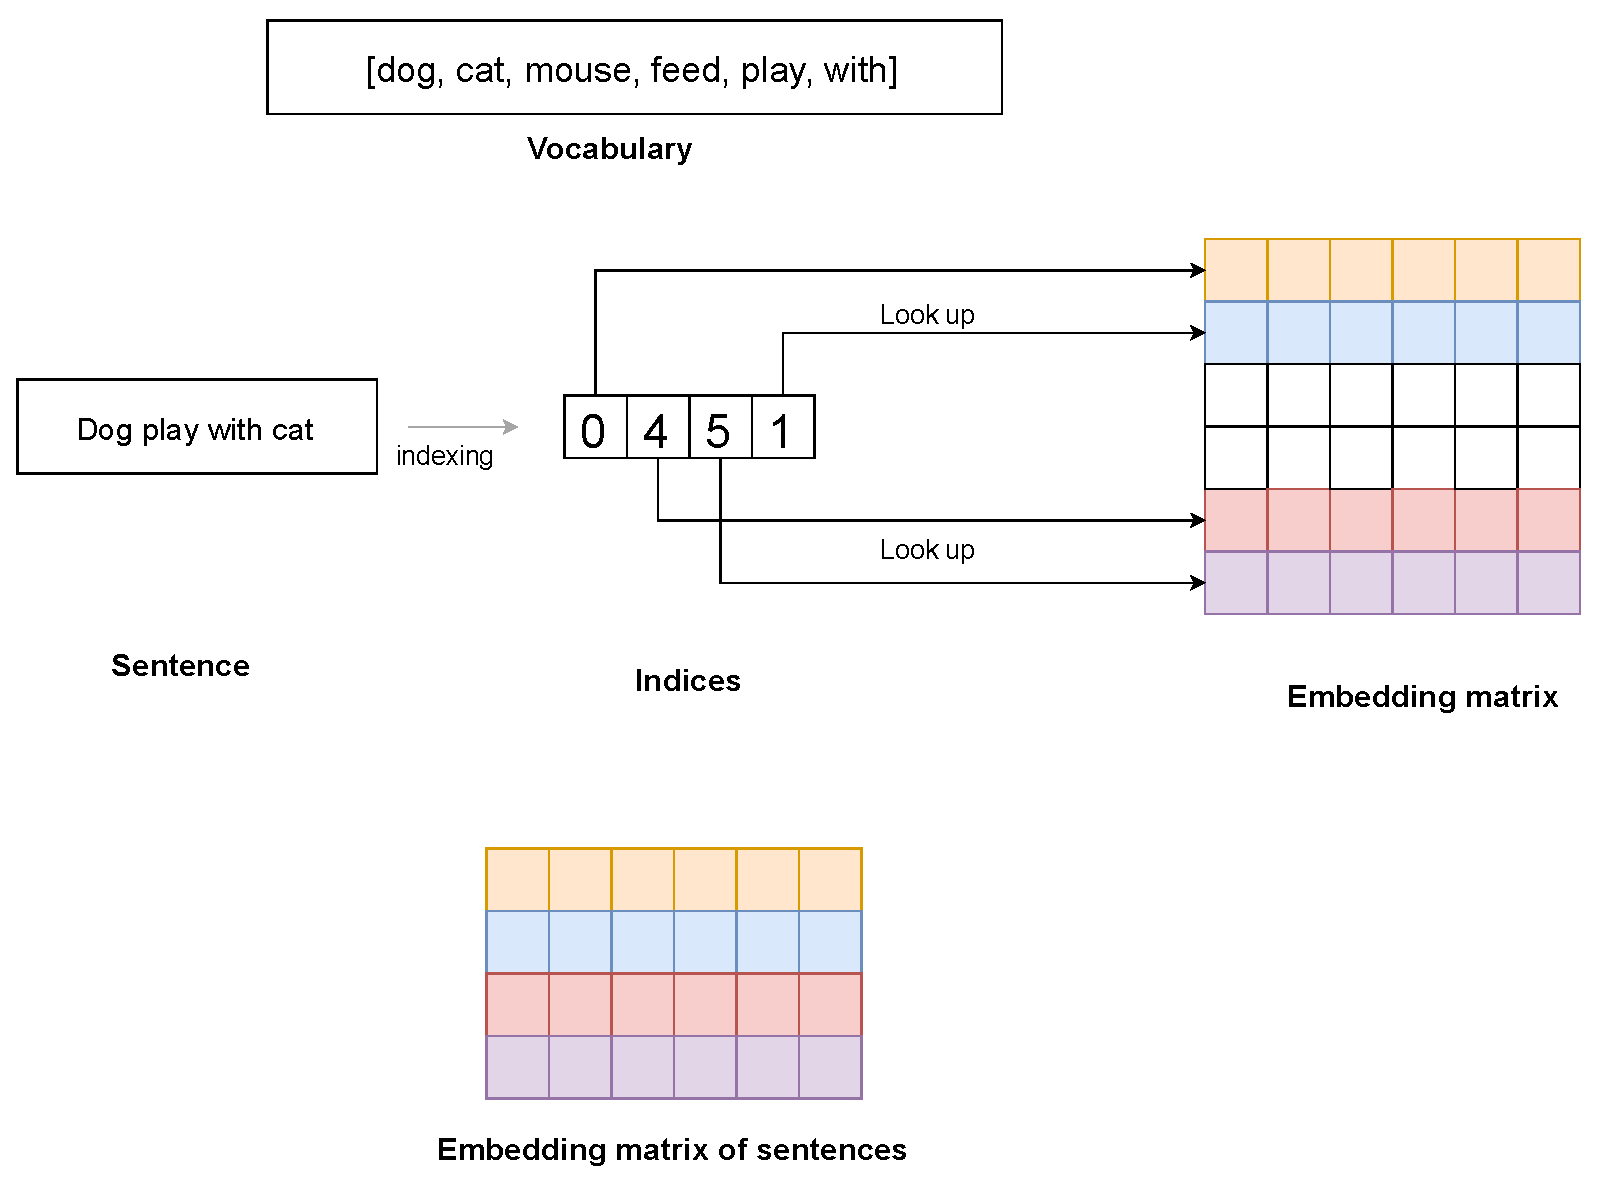
\includegraphics[width=0.9\linewidth]{figure/embeddinglayer.pdf}
	\caption[Overview of embedding layer]{Overview of Embedding Layer}
	\label{fig:embeddinglayer}
\end{figure}



\subsubsection{VT Tree-GRU}
We apply both tree structure network and recurrent structure in our model. In each sub-tree, which consist of one parent node with or without children, we apply recurrent network structure over current node and all its child. We store last hidden layer as node intermediate information and use as input to higher level. For network unit, we choose Gated Recurrent Unit (GRU), which was first introduced in \cite{cho2014learning}. GRU transition equation are describe in eq \ref{eq:gru}. 

\begin{equation}
\label{eq:gru}
\begin{aligned}
&r = sigmoid(W_{ir} x + b_{ir} + W_{hr} h + b_{hr}) \\
&i = sigmoid(W_{ii} x + b_{ii} + W_{hi} h + b_{hi}) \\
&n = \tanh(W_{in} x + b_{in} + r * (W_{hn} h + b_{hn})) \\
&h' = (1 - i) * n + i * h\\
\end{aligned}
\end{equation}

\subsubsection{Constituency VT Tree-GRU} \label{sec:VTtreeConstituency}
SST (See \ref{sec:sst}) given format is binary constituency parse tree. We use CoreNLP \cite{manning2014stanford} to create non-binary constituency parse tree and annoted Part-of-speech tag (POS-tag) for each node. We use word and tag and tree structure as input for our model.

For each sub-tree, we sort child node from left to right order. We take node state k, node POS-tag, and parent POS-tag as input for GRU timestep. We put parent node at the end of GRU chain. We take hidden state of last timestep as node state k for parent node. For a sub tree fig \ref{fig:treecp}, model is illustrate in \ref{fig:cvtgru}. For leaf node case, we input word and tag into GRU and get hidden output h as k for leaf node as fig \ref{fig:gruleaf}.
\begin{figure}[H]
	\centering
	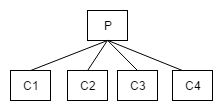
\includegraphics[width=0.5\linewidth]{figure/treecp}
	\caption[A sub tree with parent and children node]{A sub tree with parent and children node}
	\label{fig:treecp}
\end{figure}

\begin{figure}[H]
	\centering
	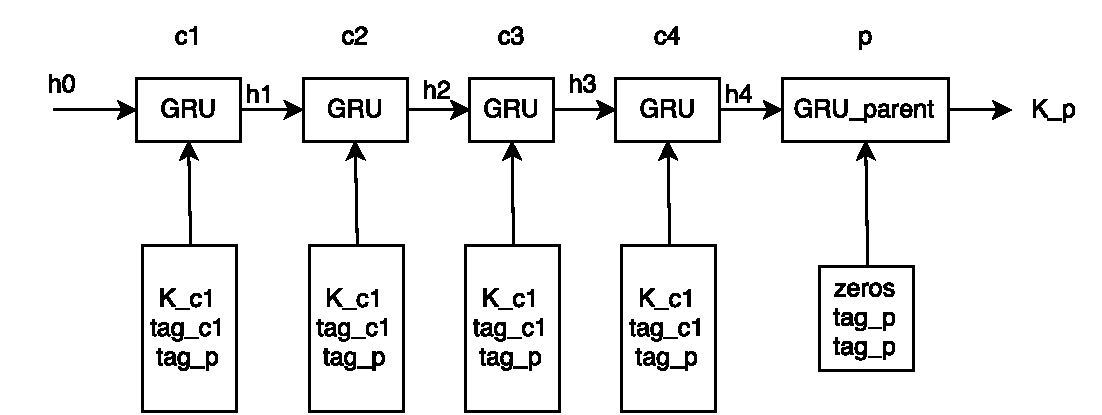
\includegraphics[width=0.9\linewidth]{figure/cvtgru}
	\caption[Constituency VT Tree-GRU]{Constituency VT Tree-GRU}
	\label{fig:cvtgru}
\end{figure}

\begin{figure}[H]
	\centering
	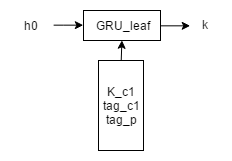
\includegraphics[width=0.4\linewidth]{figure/gruleaf}
	\caption[Constituency VT Tree-GRU leaf case]{Constituency VT Tree-GRU leaf case}
	\label{fig:gruleaf}
\end{figure}



\subsubsection{Dependency VT Tree-GRU} \label{sec:VTtreeDependency}
We use \cite{manning2014stanford} to create dependency parse tree with annoted POS-tag and labeled Universal Dependencies between head word and its dependents.

We build a model similar to constituency case, with a chain GRU for each sub tree. However, we does not put parent node at the end of the chain. Instead, parent node and child node are sorted according to their position in sentences. We take node state k, node POS-tag, node dependency relationship type vs head word as input for GRU timestep. At parent node, we set dependency relationship type is 'self' and node states k set to zeros vector. We take hidden state of last timestep as node state k for parent node. In case of leaf node, we treat it as parent node without children. We build GRU chain with only parent node for leaf case. Fig \ref{fig:dependencyvtgru} illustrate Dependency VT GRU model.

\begin{figure}[H]
	\centering
	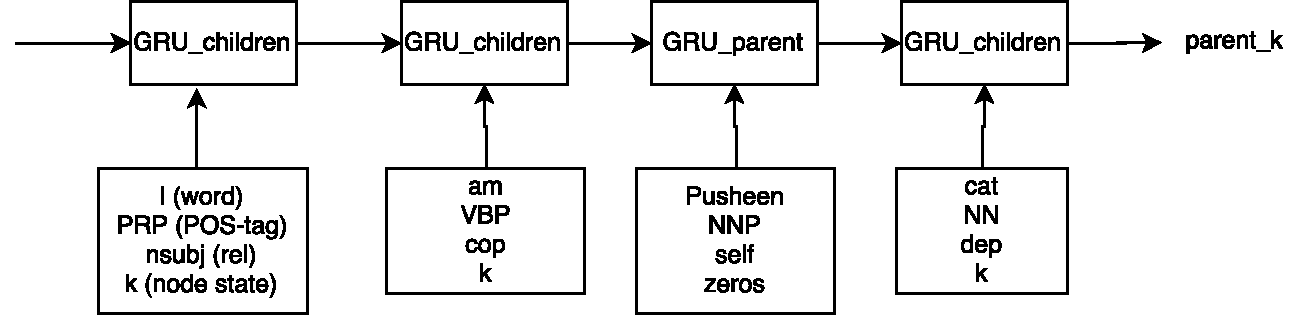
\includegraphics[width=0.9\linewidth]{figure/dependencyvtgru}
	\caption[Dependency VT Tree-GRU]{Dependency VT Tree-GRU}
	\label{fig:dependencyvtgru}
\end{figure}

\subsubsection{Output layer and loss function}
We use softmax classifier and cross entropy loss function as described in \cite{treeLSTM}.  For each parent labeled node, we use node state $k$ as input to output layer and calculate loss against given label. Root node state $k$ is used to determine sentiment of whole sentences.

\subsubsection{Training method and hyper-parameter}
We preprocess SST as described in \ref{sec:VTtreeConstituency} and \ref{sec:VTtreeDependency}. We use default train/dev/test split after remove neutral sentences (6920/872/1821). We only remove neutral sentence, but keep neutral text span of positive or negative sentences. We fine tune our model on development dataset using gird search.

We initialized our word representation with pretrained word vector (Glove \footnote{Common Crawl (840B tokens, 2.2M vocab, cased, 300d vectors, 2.03 GB download) publicly available at \url{https://nlp.stanford.edu/projects/glove/}} \cite{glove}, paragram\_xxl \footnote{50,000 embeddings, publicly available at \url{http://ttic.uchicago.edu/~wieting/}} \cite{wieting2015towards}) with default dimension of 300.  We initialize randomly tag and relationship representation (dependency only) vector of dimension 50. We set memory dimensions of 150. 

Our model was trained using AdaGrad \cite{duchi2011adaptive} with learning rate of $\{0.1,~ 0.05,~ 0.01\}$ and Adam $\{1e^{-3}, 1e^{-4}\}$, L2 regularization strength of $\{1e^{-3},~ 1e^{-4}, ~ 1e^{-5} \}$, batch size of 25. We manually update our word representation with learning rate $\alpha$ of $\{0.1,~0.05, ~0.01\}$ as equation \ref{eq:manuallyupdate}. In addition, we used dropout \cite{krizhevsky2012imagenet} to regularize our model. We regularized Tree-GRU with input dropout rate of 0.5 and memory dropout rate at 0.1. Sentiment classifier was also regularized with 0.5 dropout rate. 


\begin{equation}
\label{eq:manuallyupdate}
w = w - \alpha\delta J(\theta)
\end{equation}


\subsection{CNN-TreeLSTM}\label{sec:CNNtree}

\begin{figure}[H]
	\centering
	
\includegraphics[width=0.8\linewidth]{figure/convtreelstmsummary}
	\caption[Convolution Tree-LSTM overview]{Convolution Tree-LSTM overview}
	\label{fig:convtreelstmsummary}
\end{figure}

CNN-TreeLSTM is a combination of Convolution Neural Network with Tree-LSTM \cite{treeLSTM}. We keep embedding layer, output layer and Tree-LSTM as same as TreeLSTM implementation. We also replace Tree-LSTM with LSTM for comparison. Our CNN LSTM model are difference from \ref{cnn-rnn} as we do not use max-pooling layer, our kernel size are different with 'half' convolution strategy instead of 'valid'. We keep our model similar to \cite{treeLSTM}.

\subsubsection{Convolution layer} \label{sec:conv1c}
Each convolution layer contain n filter. Each filter has dimension $w x d$, with d is word vector dimensions and w is word-level kernel size. We may have one or more kernel size, with are treat as model hyper-parameter. 

We align the first axis of each feature map with the embedding axis and convolve along first dimension of embedding matrix. 
We use 'half' convolutions~\footnote{'half' padding policy: http://deeplearning.net/software/theano/tutorial/conv\_arithmetic.html} with unit strides, which each filter produce a 1d vector have same length as sentence length. 
Thus, n filter produces $l x n$ matrix with $l$ is sentence length. We set $n = d$ in order to produce output with same dimension as embedding matrix. We use ReLU activation function \cite{hahnloser2000digital}. Fig \ref{fig:convlayer} illustrates convolution process. 



\begin{figure}[H]
	\centering
	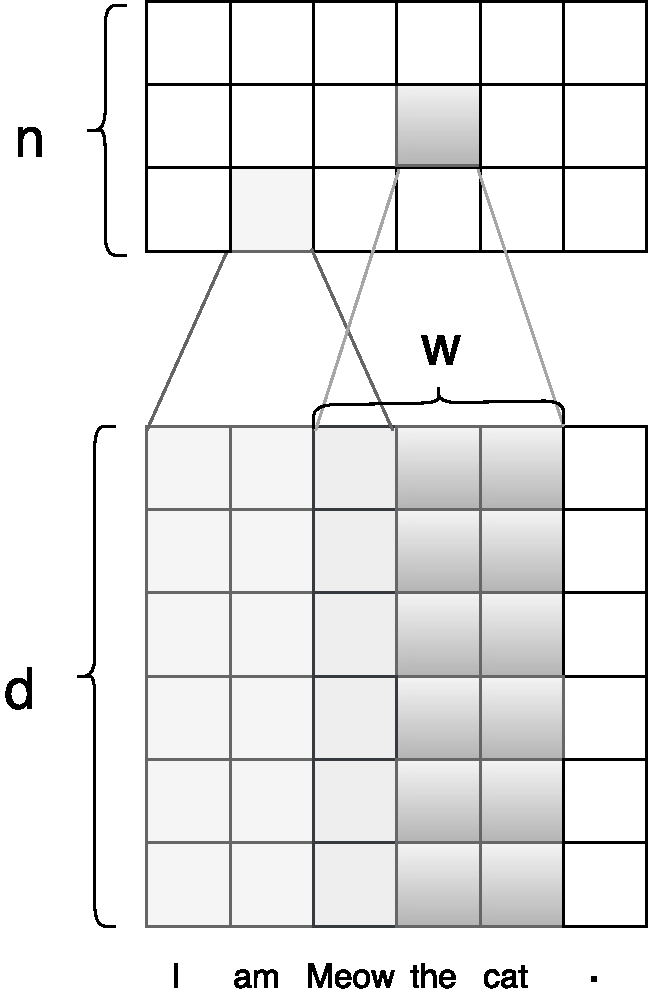
\includegraphics[width=0.6\linewidth]{figure/convlayer}
	\caption[Convolution layer]{Convolution layer}
	\label{fig:convlayer}
\end{figure}

\subsubsection{Two input channel Convolution layer} \label{sec:conv2c}
We adapt convolution layer in \ref{kim-cnn}, allowing two parallel embedding layer in our model. In other words, each word have two vector representation. The method allows two pre-trained word representation. 

\begin{figure}[H]
	\centering
	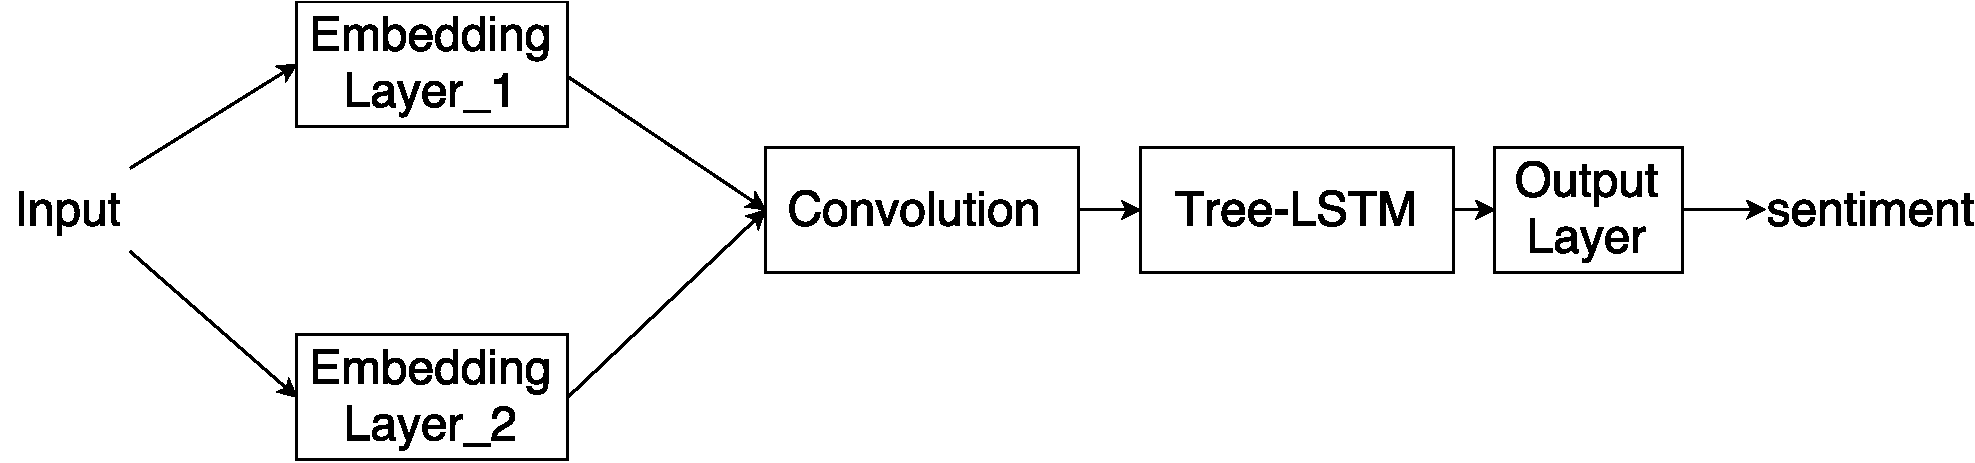
\includegraphics[width=0.8\linewidth]{figure/multichannelcnnlstm}
	\caption[Convolution Tree-LSTM overview]{Two input channel Convolution Tree-LSTM overview}
	\label{fig:multichannelcnnlstm}
\end{figure}

\subsubsection{Training method and hyper-parameter}
We train and evaluate on SST standard split train/dev/test after remove neutral sentences. We keep neutral text span for non-neutral sentences, however. We initialize word representation with Glove \footnote{\label{glovecommoncrawl}Common Crawl (840B tokens, 2.2M vocab, cased, 300d vectors, 2.03 GB download) publicly available at \url{https://nlp.stanford.edu/projects/glove/}} \cite{glove}. With two channel convolution, we initialize word representation using Glove Common Crawl and our word vector trained using Glove on Amazon dataset (Section \ref{sec:gloveamazone}). 

We tried a variety of convolution filters combination. For single kernel size, we performed gird search on $\{100, 200, 300\}$ kernel of size $\{3, 5\}$. For two different kernel size, we tried with $\{100, 200\}$ number of filter for each filter kernel size. Output matrix of different kernel size was concatenated as it was with same kernel size. 

Our model was trained using AdaGrad \cite{duchi2011adaptive} with learning rate of $\{0.1,~ 0.05,~ 0.01\}$, L2 regularization of $\{1e^{-3},~ 1e^{-4}, ~ 1e^{-5} \}$, batch size of 25. We manually update our word representation with learning rate $\alpha$ of $\{0.1,~0.05, ~0.01\}$ as equation \ref{eq:manuallyupdate}. We regularized convolution layer with input dropout rate of 0.5 and output dropout rate of 0.2 in addition to dropout of rate 0.5 at dropout layer. 

We apply same gird search parameters for two channel convolution. 


\section{Improving continuous distributed word presentation} \label{sec:improveembedding}

\subsection{Preprocess Amazon dataset}
\subsubsection{For Glove}\label{sec:preprocessamazonglove}

\begin{enumerate}
	\item We extract reviewText and overall from review dataset. We assume that overall valus are sentiment score for reviews. Reviews with overall 5 is very positive and 0 is very negative. We keep asin, reviewText, overall and omit other data points.
	\item We group dataset by product (reviews with same asin). Then for each product, we sorted by overall.
	\item We dump all reviewText into plain text file.
	\item We tokenized using Stanford Tokenizer \cite{tokenizerpart}.
\end{enumerate}

\subsubsection{For word language model}
% Preprocess procedure for %TODO: For what ?.
\begin{enumerate}
	\item We extract reviewText and overall from review dataset. We assume that overall values are sentiment score for reviews. Reviews with overall 5 is very positive and 0 is very negative. We keep reviewText, overall and omit other data points.
	\item We classify dataset reviewText into 3 classes based on overall, with 4, 5 are positive, 3 is neutral and 1, 2 are negative.
	\item For each review, we use regex to separate ending punctuation between sentences because tokenizer cannot distinct two sentences if there are not space between ending punctuation and next sentences. For example, we replace "I love cats.Cats are awesome." with "I love cats. Cats are awesome." 
	\item We tokenize dataset with Stanford Tokenizer \cite{tokenizerpart}.
\end{enumerate}

\subsection{Training Glove embedding on Amazon reviews data set}\label{sec:gloveamazone}

We use Glove implementation \footnote{Publicly available on Github \url{https://github.com/stanfordnlp/GloVe}} to train word representation. We set $x_max = 100$, vector size of 300 and windows size of 20 to train Amazon review dataset in \ref{sec:preprocessamazonglove}. We get 1,734,244 vocabularies in pre-trained word vectors. 

\subsection{Word language model}
We use Word Language model implementation \footnote{PyTorch Example \url{https://github.com/pytorch/examples/tree/master/word_language_model}} to pre-train CNN layer. We modified the code to add convolution layer as describe in Section \ref{sec:conv1c} and Section \ref{sec:conv2c}. We keep the encoder (embedding layer \ref{sec:embedding}) and decoder (word classifier). 

Each iteration, model takes 35 words at input and predicts the next word. Then the windows shift one word. Fig. \ref{fig:wordlanguagemodel} illustrates the process.

\begin{figure}[H]
	\centering
	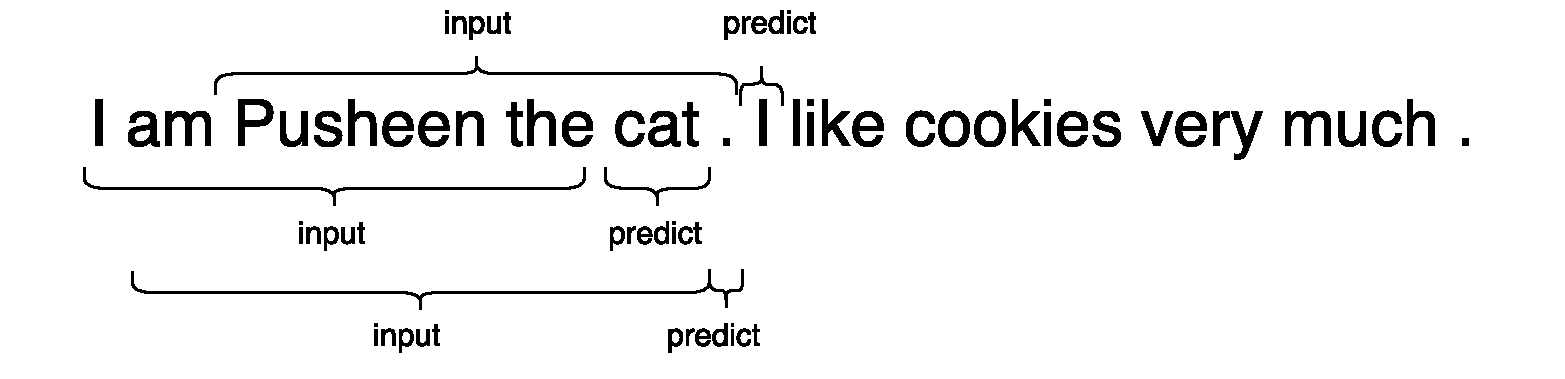
\includegraphics[width=0.9\linewidth]{figure/wordlanguagemodel}
	\caption[Word language model]{Word language model with input window size of 4}
	\label{fig:wordlanguagemodel}
\end{figure}

\subsubsection{Training method and hyper-parameter}
We initialize word vector with Glove Common Crawl and Glove Amazon Reviews pre-trained word vector. We set embedding vector size of 300, memory size of 150. We keep everything else as default setting.

%\subsection{Using hierarchical CNN to improve Glove embedding}

%\subsubsection{Training method and hyper-parameter}


%\section{Combining better sentence composition and distributed word presentation}

%\subsubsection{Training method and hyper-parameter}
